% FlightlyVR -- literature review template
% Build: pdflatex main && bibtex main && pdflatex main && pdflatex main
% TODO markers (\todo{...}) show what is left to write, in red.
% For the final version set \showtodosfalse below: they disappear.

\documentclass[11pt,a4paper]{article}

\usepackage[T1]{fontenc}
\usepackage[utf8]{inputenc}
\usepackage{lmodern}
\usepackage[margin=2.5cm]{geometry}
\usepackage{microtype}
\usepackage{booktabs}
\usepackage{tabularx}
\usepackage{longtable}
\usepackage{pdflscape}
\usepackage{array}
\usepackage{amssymb}
\usepackage{xcolor}
\usepackage{graphicx}
\usepackage{enumitem}
\usepackage[numbers,sort&compress]{natbib}
\newif\ifshowtodos \showtodostrue
\newcommand{\todo}[2][]{\ifshowtodos{\color{red}\footnotesize[TODO: #2]}\fi}
\usepackage{tikz}
\usetikzlibrary{positioning,arrows.meta}
\usepackage[hidelinks]{hyperref}

% Feature marks for the comparison table
\newcommand{\yes}{\ding{51}}
\newcommand{\no}{--}
\newcommand{\partly}{$\circ$}
\usepackage{pifont}

\newcommand{\system}{FlightlyVR}
\newcolumntype{Y}{>{\raggedright\arraybackslash}X}

\title{Immersive Exploration of Air Traffic Networks:\\
  A Literature Review of Network, Geographic, Temporal\\
  and Voice-Based Immersive Analytics}
\author{Alper Erdo\u{g}an\\
  Polytech Angers -- Projet 5A SAGI ``Data Exploration''\\
  \small Supervisor: Paul Richard}
\date{\today}

\begin{document}
\maketitle

\begin{abstract}
\todo[inline]{150--250 words. Context (immersive analytics of networks), the gap
(geographic + temporal networks with real-time voice interaction), method (number of
papers, sources, years), main findings per theme, research gaps that motivate \system.}
\end{abstract}

\noindent\textbf{Keywords:} immersive analytics; network visualization; virtual reality;
flow maps; air transport networks; natural language interfaces; large language models.

% ---------------------------------------------------------------------------
\section{Introduction}
\label{sec:intro}

Immersive analytics studies how virtual and augmented reality can support data
understanding and decision making~\cite{marriott2018immersive,ens2021grand}.
Node-link networks are one of its most studied data types~\cite{joos2025survey}.
\todo{Motivation: why air traffic networks, why VR, why voice. One paragraph each.}

\paragraph{Scope.} This review covers work at the intersection of
(i)~immersive network visualization,
(ii)~geographic flow visualization in VR,
(iii)~dynamic (time-varying) networks, and
(iv)~speech and natural language interaction for visualization,
with air transport networks as the application domain.

\paragraph{Research questions.}
\begin{enumerate}[label=\textbf{RQ\arabic*}, leftmargin=*]
  \item Which layouts (3D, egocentric, geographic) have been evaluated for networks in VR,
        and with which results?
  \item How have geographic flows (origin--destination data) been shown in immersive
        environments?
  \item How is time represented and navigated in immersive network visualization?
  \item How have speech, natural language and LLM-based assistants been used to interact
        with (immersive) visualizations, and how were they evaluated?
  \item Which gaps remain for geographic, temporal networks explored with real-time voice?
\end{enumerate}

\paragraph{Contributions.} \todo{Taxonomy / comparison table, identified gaps, positioning
of \system.}

\paragraph{Related surveys.} Earlier surveys cover immersive analytics in
general~\cite{fonnet2021survey}, abstract 3D visualizations~\cite{kraus2022survey},
open challenges~\cite{ens2021grand} and immersive network analysis~\cite{joos2025survey}
(Section~\ref{sec:surveys}).
\todo{What this review adds over them (domain: air transport; voice/LLM; time).}

% ---------------------------------------------------------------------------
\section{Review Method}
\label{sec:method}

The review follows the guidelines of Kitchenham and Charters~\cite{kitchenham2007guidelines}
and reports the selection with a PRISMA 2020 flow diagram~\cite{page2021prisma}.

\subsection{Sources and search strings}

\begin{table}[h]
\centering
\small
\begin{tabularx}{\linewidth}{lY}
\toprule
Source & Search string / note \\
\midrule
IEEE Xplore      & \texttt{("virtual reality" OR immersive OR "head-mounted") AND (graph OR network OR "node-link")} \\
ACM DL           & same \\
Eurographics DL  & same (EuroVis, PacificVis, CGF) \\
Scopus           & same, plus \texttt{AND (flight OR "air transport" OR aviation)} \\
arXiv (cs.HC, cs.GR) & preprints from 2024 on (fast-moving LLM / voice topics) \\
Snowballing      & backward and forward from \cite{joos2025survey,kraus2022survey} \\
\bottomrule
\end{tabularx}
\caption{Sources and search strings.}
\todo{Date of each search.}
\label{tab:sources}
\end{table}

\subsection{Inclusion and exclusion criteria}
\begin{itemize}[leftmargin=*]
  \item[\textbf{I1}] Peer-reviewed paper or preprint, in English, 2005--2026.
  \item[\textbf{I2}] Presents or evaluates a visualization of network, flow or geographic data
        in VR/AR, or speech / natural language interaction with a visualization.
  \item[\textbf{E1}] Desktop-only work without a transferable finding (kept only as background).
  \item[\textbf{E2}] Medical / molecular 3D rendering without network structure.
  \item[\textbf{E3}] Short abstracts without results; duplicates (keep the longest version).
\end{itemize}

\subsection{Selection}

\begin{figure}[h]
\centering
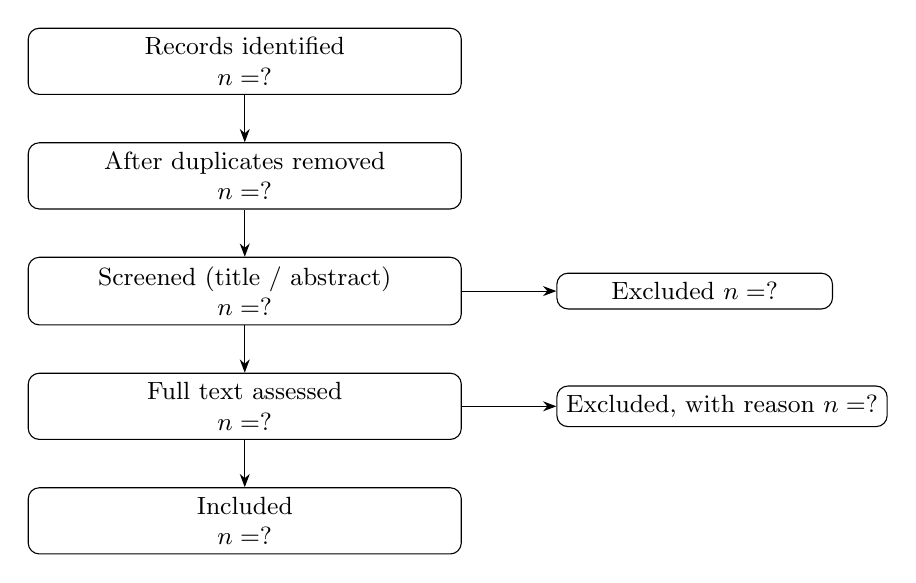
\begin{tikzpicture}[node distance=6mm, every node/.style={draw, rounded corners,
  align=center, font=\small, minimum width=5.5cm}, >={Stealth}]
  \node (id)   {Records identified\\ $n = ?$};
  \node (dup)  [below=of id]   {After duplicates removed\\ $n = ?$};
  \node (scr)  [below=of dup]  {Screened (title / abstract)\\ $n = ?$};
  \node (full) [below=of scr]  {Full text assessed\\ $n = ?$};
  \node (inc)  [below=of full] {Included\\ $n = ?$};
  \node (ex1)  [right=12mm of scr,  minimum width=3.5cm] {Excluded $n = ?$};
  \node (ex2)  [right=12mm of full, minimum width=3.5cm] {Excluded, with reason $n = ?$};
  \draw[->] (id) -- (dup); \draw[->] (dup) -- (scr); \draw[->] (scr) -- (full);
  \draw[->] (full) -- (inc); \draw[->] (scr) -- (ex1); \draw[->] (full) -- (ex2);
\end{tikzpicture}
\caption{PRISMA-style selection flow.}
\todo{Fill in the counts.}
\label{fig:prisma}
\end{figure}

\subsection{Coding scheme}
Each included paper is coded on: data type (abstract network / geographic / dynamic),
layout (2D, 3D, egocentric, map, globe), display (HMD, CAVE, AR), interaction (controller,
gesture, gaze, speech, LLM), tasks (following the graph task
taxonomy of Lee et al.~\cite{lee2006task}), evaluation (none, case study, controlled study;
$N$; measures such as SUS~\cite{brooke1996sus}, NASA-TLX~\cite{hart1988nasatlx},
SSQ~\cite{kennedy1993ssq}) and main finding.
\todo{Who coded, how disagreements were resolved.}

% ---------------------------------------------------------------------------
% Each source: one paragraph with the problem it addresses, its method and its results.
\newcommand{\src}[1]{\paragraph{#1}}
\newcommand{\prob}{\textit{Problem.}~}
\newcommand{\meth}{\textit{Method.}~}
\newcommand{\res}{\textit{Results.}~}

\section{Surveys and Research Agendas}
\label{sec:surveys}

\src{Marriott et al.~\cite{marriott2018immersive} (2018).}
\prob Immersive analytics was emerging as a field without a shared definition, vocabulary
or research agenda.
\meth Edited book with chapters by researchers from visualization, VR/AR and HCI, each
covering one aspect (definitions, interaction, collaboration, evaluation, applications).
\res Defines immersive analytics as the use of engaging, embodied analysis tools to
support data understanding and decision making, and sets out the open questions that later
work builds on.
\todo{Check the definition wording against the book's first chapter.}

\src{Fonnet and Pri\'e~\cite{fonnet2021survey} (2021).}
\prob Immersive data analysis systems had been built for three decades, but no survey
covered them.
\meth Survey of immersive analytics systems from the early 1990s to 2019, classified by
rendering technology, data, sensory mapping, interaction and evaluation.
\res Multi-sensory aspects are under-used, knowledge from the 3D user interface and VR
communities is not applied enough, the field should converge on best practices and aim for
real-life systems.

\src{Kraus et al.~\cite{kraus2022survey} (2022).}
\prob Publications on abstract (non-spatial) data in immersive environments had grown
quickly but were hard to compare.
\meth EuroVis state-of-the-art report: a characterization along the use of 3D, embedding
in the immersive space, combination with spatial data, interaction paradigms and
evaluation, applied to the published works.
\res Overview of the state of the art, current trends, and gaps and challenges; the
characterization serves as a frame to position new systems.

\src{Ens et al.~\cite{ens2021grand} (2021).}
\prob A fast-moving field spread over many venues needed a common research agenda.
\meth 24 international experts, starting from a virtual workshop at ACM CHI 2020, developed
challenges over several sessions.
\res 17 grand challenges forming a roadmap, among them natural and multimodal interaction
and evaluation with real data and users.

\src{Joos et al.~\cite{joos2025survey} (2025).}
\prob Immersive network visualization is fragmented: the design space is not described
and it is unclear which design questions are backed by evidence.
\meth Structured survey of 138 publications: design-space dimensions, their coverage in 87
applications, and 59 user evaluations; online interactive resource.
\res A design space for immersive network analysis, a synthesis of experimental findings,
key achievements and research gaps, and design guidance. It is the backbone for
Section~\ref{sec:networks}.

% ---------------------------------------------------------------------------
\section{Immersive Network Visualization}
\label{sec:networks}

\subsection{Layouts: 3D, spherical and egocentric}

\src{Kwon et al.~\cite{kwon2016study} (2016).}
\prob Information visualization had kept to 2D; layout, rendering and interaction methods
for graphs in head-mounted displays were barely explored.
\meth Design of a spherical layout with the viewer at its centre, rendering (including edge
bundling and depth cues) and interaction techniques for HMDs; user study against a
traditional 2D graph visualization.
\res Participants answered significantly faster and with fewer interactions in the
immersive condition, especially on harder tasks; overall correctness did not differ, but
was significantly higher for larger graphs.

\src{Cordeil et al.~\cite{cordeil2017cave} (2017).}
\prob Collaborative analysis of abstract data in CAVE-style rooms versus low-cost HMDs had
never been studied formally.
\meth First user study of collaborative network connectivity tasks in pairs, HMD versus the
CAVE2.
\res HMD pairs were faster; the CAVE2 led to asymmetric movement between collaborators;
accuracy and communication did not differ.

\src{Kotlarek et al.~\cite{kotlarek2020mental} (2020).}
\prob It was unclear whether an immersive view helps or hurts the mental map users build of
a network.
\meth Comparison of a 3D immersive and a 2D desktop environment on three mental-map tasks:
interpreting structure, memorizing nodes and identifying structural changes.
\res Structure was interpreted more accurately in the immersive environment, especially
for larger networks; the 2D desktop was better for tasks that need spatial memory.

\src{Sorger et al.~\cite{sorger2021egocentric} (2021).}
\prob Visual clutter and cybersickness limit exploration inside 3D networks.
\meth ``Egocentrism'' metaphor: depiction and interaction adapted to the user's position in
the network; interfaces with different degrees of egocentrism compared in a user study
(visual search, traversal efficiency, spatial orientation, cybersickness).
\res A simple egocentric interface clearly improved visual search and navigation without
reducing spatial orientation or increasing cybersickness; an occlusion-free ``Ego-Bubble''
added little. Released as an online tool.

\src{Bauer et al.~\cite{bauer2024multilayout} (2024).}
\prob Immersive network systems use one static layout, but no layout suits every task.
\meth Multi-layout system for hierarchical network data in VR that switches layouts and
interactions with the task and level of detail; user study against a state-of-the-art
immersive baseline at different spatial scopes.
\res The multi-layout approach outperformed the baseline both in spatially focused tasks
and when the whole network had to be considered.

\src{Takahira et al.~\cite{takahira2026surrounded} (2026).}
\prob Egocentric networks (an ego and its neighbours) suffer from clutter on the desktop;
layouts tailored to immersive space were missing.
\meth Design properties and dimensions for immersive egocentric layouts; four layouts
(Cube, Cylindrical, Radial, Spherical); user study with 24 participants on egocentric
analysis tasks.
\res Cube worked well for ego--alter connection strength; Spherical was more effective for
understanding the neighbours' topology, reducing occlusion and using 3D space.

\subsection{Visual encoding of edges}

\src{B\"uschel et al.~\cite{buschel2019ar} (2019).}
\prob There was little knowledge on how to draw edges in 3D node-link diagrams for
efficient immersive analysis.
\meth Exploration of the design space of edge styles in augmented reality and a user study
comparing six edge variants.
\res \todo{Add which edge styles performed best (the abstract does not say; read the
results section).}

\subsection{Navigation and embodiment}

\src{Huang et al.~\cite{huang2023embodied} (2023).}
\prob Navigating to different parts of a network quickly is essential, but the effect of
different levels of embodied interaction had not been studied.
\meth Controlled study with 20 participants and four environments, from a 2D desktop with a
mouse to 3D VR, on three navigation-heavy network tasks; accuracy, speed, workload and
preference measured.
\res On the task that required scanning the whole network, VR and a trackball mouse were
more accurate than the desktop; VR was the least mentally demanding and frustrating in two
of three tasks and the most preferred; comparing two side-by-side networks was hard in VR.

\src{Bozgeyikli et al.~\cite{bozgeyikli2016teleport} (2016).}
\prob Locomotion strongly shapes the VR experience, and continuous movement can cause
motion sickness.
\meth ``Point \& Teleport'' (point where to be, get teleported) compared with walk-in-place
and joystick; a second experiment added choosing the orientation; 16 users.
\res Point \& Teleport was fun and easy to use and has no visible translation (so it is
not expected to cause motion sickness); the added direction component degraded the
experience.

\src{Zhang et al.~\cite{zhang2025gd} (2025).}
\prob How users look at networks in VR is unknown.
\meth Eye-tracking study in VR with 18 participants relating structural properties of the
graph to gaze behaviour.
\res \todo{Verify authors, method and results from the paper; the numbers come from the
earlier report.}

% ---------------------------------------------------------------------------
\section{Geographic Flows and Air Traffic}
\label{sec:geo}

\src{Yang et al.~\cite{yang2018maps} (2018).}
\prob How to render world-wide geographic maps in VR was open.
\meth Comparison of four designs: exocentric globe, flat map, egocentric globe (viewer
inside) and curved map around the user; the geographic centre can be moved with a
controller and users can walk around; tasks on distance, area and direction.
\res The exocentric globe was most accurate for distance and most accurate and fastest for
direction, and weakly preferred; area took longer on globes than on flat and curved maps;
the curved map generally beat the flat map; the egocentric globe was the least effective.

\src{Yang et al.~\cite{yang2019flowmaps} (2019).}
\prob When displays are no longer flat, how should origin--destination flows be drawn in
the space around the user?
\meth Three studies: 2D and 3D encodings of flows on flat maps, then flat maps, 3D globes
and ``MapsLink'' (a pair of linked flat maps).
\res On flat maps, raised flows with height proportional to distance were most accurate and
straight 2D lines fastest; MapsLink was slowest; the 3D globe with raised flows was the
fastest, most accurate and most preferred. Careful use of the third dimension reduces
clutter in flow maps.

\src{Hurter et al.~\cite{hurter2019fiberclay} (2019).}
\prob Large sets of 3D trajectories (aircraft routes, brain fibres) overlap and cross,
so individual ones cannot be followed in dense areas.
\meth FiberClay renders many trajectories in real time on the GPU in VR and adds
interaction techniques that use the controllers and the user's position to compose 3D
queries.
\res Analysts can select and compare sets of trajectories by geometry and data
properties; insights are reported with domain experts in air traffic control and
neurology.

\src{Guimer\`a et al.~\cite{guimera2005worldwide} (2005).}
\prob The global structure of the air transportation network and the roles of its cities
were not understood.
\meth Network analysis of the worldwide air transportation network: degree, centrality,
community detection and each city's pattern of inter- and intra-community links.
\res The network is scale-free and small-world, but the most connected cities are not
always the most central; this comes from its multi-community structure, which geography
alone does not explain (geopolitics matters); each city gets a global role.

% ---------------------------------------------------------------------------
\section{Time-Varying Networks}
\label{sec:time}

\src{Sorger et al.~\cite{sorger2019dynamic} (2019).}
\prob Large dynamic networks are analysed in 2D, and immersive solutions scale poorly and
rely on fly- or walk-through navigation.
\meth VR system that interweaves overview exploration and immersive detail analysis, on a
web-based 3D engine supporting several input modalities.
\res Validated with a performance evaluation and an expert case study on a co-morbidity
network; no controlled user study.

\src{Filipov et al.~\cite{filipov2022time} (2023).}
\prob Structural (node-link vs.\ matrix) and temporal (animation vs.\ juxtaposition)
encodings of dynamic graphs had rarely been compared together.
\meth Study of response time, accuracy and preference for combinations of structural and
temporal encodings on typical dynamic network tasks, with and without interaction.
\res Matrices supported tasks on low-level entities better; interaction made answers
slower but more accurate; node-link with automatic animation was fastest and most accurate
overall; animation with playback control was the preferred temporal encoding.

% ---------------------------------------------------------------------------
\section{Speech, Natural Language and LLM Interaction}
\label{sec:voice}

\src{Bolt~\cite{bolt1980put} (1980).}
\prob Graphics interfaces relied on keyboards and devices; users could not simply say and
show what they wanted.
\meth ``Put-that-there'' in MIT's Media Room: speech recognition combined with pointing at
a large wall display to create, move and change objects.
\res Deictic words (``that'', ``there'') are resolved by pointing, showing that voice and
gesture together make a natural interface; a demonstration system, without a formal user
study.

\src{Srinivasan and Stasko~\cite{srinivasan2018orko} (2018).}
\prob Visualization tools are mostly WIMP-based; natural language and direct manipulation
were rarely combined, and network visualization had almost no natural language interaction.
\meth Architecture and prototype (Orko) for network visualization accepting both natural
language and touch-based direct manipulation; initial user evaluation.
\res The two modalities complement each other; observations give opportunities and
challenges for multimodal network visualization interfaces.

\src{Badam et al.~\cite{badam2017affordances} (2017).}
\prob Which input modalities suit visual data exploration in immersive environments.
\meth Workshop paper analysing the affordances of input modalities (such as touch, speech,
gesture and gaze) for immersive visual exploration.
\res \todo{Add the main recommendations from the paper.}

\src{Song et al.~\cite{song2025embodied} (2025).}
\prob How users phrase spoken requests in immersive analytics, and how they use embodiment
cues (``this'', ``here'') in speech, was underexplored.
\meth Wizard-of-Oz study with 15 participants; axial coding of 1,280 speech acts from 734
utterances; speech input uncertainty measured with semantic entropy.
\res Five speech input patterns: users blend embodied and non-embodied speech depending on
task, phase and reliance on embodiment cues; embodiment cues raise uncertainty for the
system; design implications per pattern.

\src{De La Torre et al.~\cite{delatorre2024llmr} (2024).}
\prob Creating and changing interactive mixed reality worlds in real time with LLMs fails
when training data is scarce or behaviour must be synthesized.
\meth LLMR framework on Unity: scene understanding, task planning, self-debugging and memory
management around GPT-4; evaluation on creation and modification tasks; usability study
($N = 11$).
\res About four times lower average error rate than plain GPT-4; diverse objects, tools and
scenes produced and edited; positive participant experiences.

\src{Lee et al.~\cite{lee2026voice} (2026).}
\prob Authoring operations of visual network analysis lack UI affordances in immersive
environments, and multimodal input has a steep learning curve.
\meth Research-through-design study: a system with LLM-supported voice interaction for
immersive network visualization; user study on social network analysis with participants
from social and computer science.
\res Voice raised perceived usability over controllers and lowered the effort of formulating
commands, as users stated intent in natural language; it supports complex,
multi-parameter operations. Closest work to \system{}.

% ---------------------------------------------------------------------------
\section{Methods and Instruments Used}
\label{sec:instruments}

\src{Fruchterman and Reingold~\cite{fruchterman1991graph} (1991).}
\prob Drawing undirected graphs with straight edges in a readable way.
\meth Modification of Eades' spring embedder: forces modelled on natural systems, aiming at
uniform edge lengths.
\res A simple, intuitive and efficient force-directed algorithm; used by \system{} for the
3D shell layout.

\src{Blondel et al.~\cite{blondel2008louvain} (2008).}
\prob Community detection methods were too slow for very large networks.
\meth Heuristic modularity optimization (the ``Louvain'' method).
\res Faster than all other known methods with high modularity; shown on a 2-million-customer
phone network and a 118-million-node web graph; used by \system{} for regional clusters.

\src{Lee et al.~\cite{lee2006task} (2006).}
\prob Designers and evaluators of graph visualizations lacked a detailed, shared task list.
\meth Definition of graph-specific objects and a list of commonly encountered tasks.
\res Complex tasks can be described as series of low-level tasks on those objects; the
taxonomy supports comparable controlled experiments. Basis of the study tasks.

\src{Brooke~\cite{brooke1996sus} (1996).}
\prob Industry needed a quick, reliable usability measure.
\meth System Usability Scale: ten statements on a five-point agreement scale.
\res A single 0--100 usability score, now the most widely used usability questionnaire.

\src{Hart and Staveland~\cite{hart1988nasatlx} (1988).}
\prob Measuring the mental workload of operators.
\meth Development of the NASA Task Load Index from empirical and theoretical research: six
subscales (mental, physical and temporal demand, performance, effort, frustration) with
pairwise weighting.
\res A multidimensional workload score, standard in HCI and VR studies.

\src{Kennedy et al.~\cite{kennedy1993ssq} (1993).}
\prob The motion sickness questionnaire in use did not fit simulator sickness.
\meth Factor analyses of more than 1,100 questionnaires from 10 Navy simulators, validated
on 3,691 simulator flights.
\res The Simulator Sickness Questionnaire with simple scoring and better diagnostic power;
used to measure cybersickness in VR.

\src{Kitchenham and Charters~\cite{kitchenham2007guidelines} (2007).}
\prob Literature reviews in computing were often unsystematic and not reproducible.
\meth Guidelines adapted from medical research for planning, conducting and reporting
systematic reviews.
\res A protocol (research questions, search strategy, selection, quality assessment, data
extraction) followed in Section~\ref{sec:method}.

\src{Page et al.~\cite{page2021prisma} (2021).}
\prob The 2009 PRISMA statement was outdated by advances in review methods.
\meth Updated guideline built by an expert group.
\res A 27-item checklist, an abstract checklist and new flow diagrams; used for
Figure~\ref{fig:prisma}.

% ---------------------------------------------------------------------------
\section{Comparison}
\label{sec:comparison}

Table~\ref{tab:detail} compares the 22 primary studies of
Sections~\ref{sec:networks}--\ref{sec:voice} on data, display, encoding, interaction,
evaluation and main finding; Table~\ref{tab:features} summarises which aspects each covers
next to \system{}; Table~\ref{tab:surveys} compares the five surveys of
Section~\ref{sec:surveys}. The methods and instruments of Section~\ref{sec:instruments} are
not compared. $N$ = participants; ``?'' = not given in the abstract.
\todo{Fill every ``?'' from the papers' method sections.}

\begin{landscape}
\footnotesize
\setlength{\tabcolsep}{3pt}
\renewcommand{\arraystretch}{1.15}
\begin{longtable}{>{\raggedright\arraybackslash}p{2.9cm}
                  >{\raggedright\arraybackslash}p{2.3cm}
                  >{\raggedright\arraybackslash}p{2.0cm}
                  >{\raggedright\arraybackslash}p{3.0cm}
                  >{\raggedright\arraybackslash}p{2.4cm}
                  >{\raggedright\arraybackslash}p{2.6cm}
                  >{\raggedright\arraybackslash}p{6.4cm}}
\caption{Detailed comparison of the primary studies.}\label{tab:detail}\\
\toprule
Work & Data & Display & Layout / encoding & Interaction & Evaluation ($N$) & Main finding \\
\midrule
\endfirsthead
\multicolumn{7}{l}{\textit{Table~\ref{tab:detail} continued}}\\
\toprule
Work & Data & Display & Layout / encoding & Interaction & Evaluation ($N$) & Main finding \\
\midrule
\endhead
\midrule
\multicolumn{7}{r}{\textit{continued on next page}}\\
\endfoot
\bottomrule
\endlastfoot
\multicolumn{7}{l}{\textbf{Immersive network visualization}}\\
Kwon et al.~\cite{kwon2016study} 2016 & Abstract graphs & HMD vs.\ 2D desktop & Spherical layout, viewer at centre; edge bundling & Head tracking, controller & Controlled study (?) & Faster, fewer interactions in VR on hard tasks; more correct on large graphs \\
Cordeil et al.~\cite{cordeil2017cave} 2017 & Abstract networks & HMD vs.\ CAVE2 & 3D node-link & Collaborative, physical movement & Controlled study, pairs (?) & HMD faster; CAVE2 asymmetric movement; same accuracy and communication \\
Kotlarek et al.~\cite{kotlarek2020mental} 2020 & Abstract networks & HMD vs.\ 2D desktop & 3D vs.\ 2D node-link & Not specified & Controlled study (?) & VR better for structure (large networks); desktop better for spatial memory \\
Sorger et al.~\cite{sorger2021egocentric} 2021 & Abstract networks & HMD & Egocentric view, Ego-Bubble & Egocentric navigation & Controlled study (?) & Egocentric interface improves search and navigation, no extra cybersickness \\
Bauer et al.~\cite{bauer2024multilayout} 2024 & Hierarchical networks & VR HMD & Multiple switchable layouts & Layout switching & Controlled study vs.\ baseline (?) & Beats baseline for focused and whole-network tasks \\
Takahira et al.~\cite{takahira2026surrounded} 2026 & Egocentric networks & Immersive HMD & Cube, cylindrical, radial, spherical & Not specified & Controlled study (24) & Cube best for tie strength; spherical best for topology, least occlusion \\
B\"uschel et al.~\cite{buschel2019ar} 2019 & 3D node-link & AR & Six edge styles & Not specified & Controlled study (?) & ? (results not in abstract) \\
Huang et al.~\cite{huang2023embodied} 2023 & Networks & Desktop (mouse, trackball) to VR & 2D vs.\ 3D & Four levels of embodiment & Controlled study (20) & VR least demanding, most preferred; side-by-side comparison hard in VR \\
Bozgeyikli et al.~\cite{bozgeyikli2016teleport} 2016 & -- (locomotion) & HMD & -- & Point \& Teleport vs.\ walk-in-place vs.\ joystick & Two experiments (16) & Teleport fun and easy; adding direction choice made it worse \\
Zhang et al.~\cite{zhang2025gd} 2025 & Graphs & VR HMD, eye tracking & 3D node-link & Gaze (measured) & User study (18, unverified) & Structural properties linked to gaze (to verify) \\
\midrule
\multicolumn{7}{l}{\textbf{Geographic flows and air traffic}}\\
Yang et al.~\cite{yang2018maps} 2018 & World maps & VR HMD & Exocentric globe, flat map, egocentric globe, curved map & Controller (move centre), walking & Controlled study (?) & Exocentric globe best for distance and direction; curved beats flat; egocentric globe worst \\
Yang et al.~\cite{yang2019flowmaps} 2019 & Global OD flows & VR HMD & 2D/3D flows on flat maps, globes, MapsLink & Controller, walking & Three controlled studies (?) & Globe with raised flows fastest, most accurate, preferred; raised flows help on flat maps \\
Hurter et al.~\cite{hurter2019fiberclay} 2019 & 3D trajectories (air traffic, brain fibres) & VR HMD & Massive 3D lines (GPU) & 3D query composition with controllers and body position & Expert feedback (?) & Analysts select and compare trajectory sets; insights with air traffic controllers \\
Guimer\`a et al.~\cite{guimera2005worldwide} 2005 & Worldwide air transport network & -- & -- & -- & Network analysis & Scale-free small world; hubs not always central; communities not only geographic \\
\midrule
\multicolumn{7}{l}{\textbf{Time-varying networks}}\\
Sorger et al.~\cite{sorger2019dynamic} 2019 & Large dynamic network & VR HMD (web-based) & Overview + immersive detail & Multiple input modalities, time navigation & Performance test, expert case study & Scales to large dynamic graphs; no controlled study \\
Filipov et al.~\cite{filipov2022time} 2023 & Dynamic graphs & Desktop & Node-link vs.\ matrix; animation vs.\ juxtaposition & With / without interaction & Controlled study (?) & Node-link with auto animation fastest and most accurate; playback control preferred \\
\midrule
\multicolumn{7}{l}{\textbf{Speech, natural language and LLM interaction}}\\
Bolt~\cite{bolt1980put} 1980 & Graphical objects & Wall display (Media Room) & -- & Speech + pointing & Demonstration & Deictic words resolved by pointing; voice and gesture complement \\
Srinivasan, Stasko~\cite{srinivasan2018orko} 2018 & Networks & Touch display & Node-link & Natural language + touch & Initial user study (?) & NL and direct manipulation complement each other \\
Badam et al.~\cite{badam2017affordances} 2017 & Visual data & Immersive (various) & -- & Touch, speech, gesture, gaze & Analysis (workshop paper) & ? (to add) \\
Song et al.~\cite{song2025embodied} 2025 & Visual analytics data & Immersive & -- & Speech (Wizard of Oz) & Wizard-of-Oz study (15) & Five speech patterns; embodied cues (``this'', ``here'') add uncertainty \\
De La Torre et al.~\cite{delatorre2024llmr} 2024 & MR scenes & MR (Unity) & -- & Text prompts to an LLM & Task benchmark + usability (11) & 4$\times$ lower error than GPT-4; positive usability \\
Lee et al.~\cite{lee2026voice} 2026 & Social networks & VR HMD & Node-link & LLM voice vs.\ controller & User study (?) & Voice raises perceived usability, lowers effort of forming commands \\
\midrule
\textbf{\system{}} & Air traffic network, 68 months (EUROCONTROL), OpenFlights & Quest HMD & 3D shell (force-directed, Louvain) $\leftrightarrow$ curved map of Europe & Controllers, teleport, push-to-talk voice (Wit, Gemini Live with tool calls) & Planned & -- \\
\end{longtable}
\end{landscape}

\begin{table}[p]
\centering
\small
\setlength{\tabcolsep}{4pt}
\begin{tabularx}{\linewidth}{Yccccccc}
\toprule
Work & Network & Geographic & Time & Speech/NL & LLM & Immersive & Controlled study \\
\midrule
Kwon et al.~\cite{kwon2016study}               & \yes & \no & \no & \no & \no & \yes & \yes \\
Cordeil et al.~\cite{cordeil2017cave}          & \yes & \no & \no & \no & \no & \yes & \yes \\
Kotlarek et al.~\cite{kotlarek2020mental}      & \yes & \no & \partly & \no & \no & \yes & \yes \\
Sorger et al.~\cite{sorger2021egocentric}      & \yes & \no & \no & \no & \no & \yes & \yes \\
Bauer et al.~\cite{bauer2024multilayout}       & \yes & \no & \no & \no & \no & \yes & \yes \\
Takahira et al.~\cite{takahira2026surrounded}  & \yes & \no & \no & \no & \no & \yes & \yes \\
B\"uschel et al.~\cite{buschel2019ar}          & \yes & \no & \no & \no & \no & \yes & \yes \\
Huang et al.~\cite{huang2023embodied}          & \yes & \no & \no & \no & \no & \yes & \yes \\
Bozgeyikli et al.~\cite{bozgeyikli2016teleport} & \no & \no & \no & \no & \no & \yes & \yes \\
Zhang et al.~\cite{zhang2025gd}                & \yes & \no & \no & \no & \no & \yes & \yes \\
Yang et al.~\cite{yang2018maps}                & \no & \yes & \no & \no & \no & \yes & \yes \\
Yang et al.~\cite{yang2019flowmaps}            & \partly & \yes & \no & \no & \no & \yes & \yes \\
Hurter et al.~\cite{hurter2019fiberclay}       & \no & \yes & \partly & \no & \no & \yes & \no \\
Guimer\`a et al.~\cite{guimera2005worldwide}   & \yes & \partly & \no & \no & \no & \no & \no \\
Sorger et al.~\cite{sorger2019dynamic}         & \yes & \no & \yes & \no & \no & \yes & \no \\
Filipov et al.~\cite{filipov2022time}          & \yes & \no & \yes & \no & \no & \no & \yes \\
Bolt~\cite{bolt1980put}                        & \no & \no & \no & \yes & \no & \partly & \no \\
Srinivasan, Stasko~\cite{srinivasan2018orko}   & \yes & \no & \no & \yes & \no & \no & \partly \\
Badam et al.~\cite{badam2017affordances}       & \no & \no & \no & \yes & \no & \yes & \no \\
Song et al.~\cite{song2025embodied}            & \no & \no & \no & \yes & \no & \yes & \partly \\
De La Torre et al.~\cite{delatorre2024llmr}    & \no & \no & \no & \yes & \yes & \yes & \partly \\
Lee et al.~\cite{lee2026voice}                 & \yes & \no & \no & \yes & \yes & \yes & \yes \\
\midrule
\system{}                                     & \yes & \yes & \yes & \yes & \yes & \yes & \textbf{?} \\
\bottomrule
\end{tabularx}
\caption{Aspects covered by each primary study (\yes{} yes, \partly{} partly, \no{} no).
``Controlled study'': a user study comparing conditions; \partly{} = initial, usability or
Wizard-of-Oz study without a comparison.}
\label{tab:features}
\end{table}

\begin{table}[t]
\centering
\small
\begin{tabularx}{\linewidth}{>{\raggedright\arraybackslash}p{3.2cm}YYY}
\toprule
Survey & Scope & Corpus / method & Output \\
\midrule
Marriott et al.~\cite{marriott2018immersive} 2018 & Immersive analytics (field) & Edited book, expert chapters & Definition and research agenda \\
Fonnet, Pri\'e~\cite{fonnet2021survey} 2021 & Immersive analytics systems, 1990s--2019 & Systematic survey & Rendering, data, mapping, interaction, evaluation; gaps \\
Kraus et al.~\cite{kraus2022survey} 2022 & Abstract 3D data in immersive environments & EuroVis STAR & Characterization scheme; trends and gaps \\
Ens et al.~\cite{ens2021grand} 2021 & Immersive analytics (field) & 24 experts, CHI 2020 workshop & 17 grand challenges \\
Joos et al.~\cite{joos2025survey} 2025 & Immersive network analysis & 138 papers (87 applications, 59 evaluations) & Design space, evidence synthesis, online resource \\
\bottomrule
\end{tabularx}
\caption{Comparison of the surveys.}
\label{tab:surveys}
\end{table}
\clearpage

% ---------------------------------------------------------------------------
\section{Research Gaps and Positioning}
\label{sec:gaps}

\begin{enumerate}[label=\textbf{G\arabic*}, leftmargin=*]
  \item Geographic and topological layouts of the same network have been studied separately
        (\cite{kwon2016study} vs.~\cite{yang2018maps,yang2019flowmaps}); switching between
        them in one immersive system is little explored.
  \item No controlled study compares a VR time slider for dynamic networks with an
        alternative (\cite{sorger2019dynamic} is a case study).
  \item Voice interaction for immersive networks uses speech-to-text pipelines on abstract
        social networks~\cite{lee2026voice}; real-time speech-to-speech models that call
        application tools, on geographic and temporal data, are not studied.
  \item Evaluations rarely use real, large operational datasets~\cite{ens2021grand}.
\end{enumerate}
\todo{How \system{} addresses each gap; planned user study.}

% ---------------------------------------------------------------------------
\section{Threats to Validity}
\label{sec:threats}
\todo{Search strings may miss work; preprints (arXiv) are not peer reviewed;
single coder; fast-moving LLM topic (cut-off date of the search).}

% ---------------------------------------------------------------------------
\section{Conclusion}
\label{sec:conclusion}
\todo{Answer RQ1--RQ5 in one paragraph each or one short list.}

% ---------------------------------------------------------------------------
\section*{Data Notice}
This document/R\&D product has been created with or contains elements of Aviation Data
Repository for Research made available by EUROCONTROL. \textcopyright 2020, EUROCONTROL.
EUROCONTROL does not necessarily support and/or endorse the conclusion of this
document/R\&D product.
\todo{Copy the full notice text from the EUROCONTROL terms of use (Art.~6).}

\bibliographystyle{abbrvnat}
\bibliography{refs}

\end{document}
